\section{Cost-Benefit Analysis of Clock Stability and Synchronization 
on Duty Cycling, Bandwidth, and Power Consumption}
\label{sec:power}

It is generally assumed that using a more stable clock will improve the duty
cycling capabilities of an embedded system and save bandwidth since less 
frequent resynchronizations are necessary. Dutta
showed in \cite{dutta2007procrastination} that the lower bound of a clock with
a stability of $\pm 50$ppm is a duty cycle of 0.01\% for a scheduled
communication MAC protocol. But, how much additional power and bandwidth could be saved by
employing a more stable clock, considering that a more stable clock consumes
more power? The bounds on synchronization error derived in this section along 
with the constraints on power consumption are for use in designing the applications 
on the network, such as the detector in Section \ref{sec:detector}, which uses a maximum 
synchronization error as an input parameter: $\epsilon$ for the case without 
synchronization, and $b$ for the case with synchronization algorithms.


\subsection{Clock Stability and Duty Cycling}
Let us compare two systems, $A$ and $B$. Both systems have the same sleep power
consumption $P_s$ and active power consumption $P_a$.  Each node has a local
clock source with stability $s_A$ and $s_B$ (in $Hz/Hz$) that consume power $P_{cA}$ and $P_{cB}$,
respectively. Additionally, we assume that both platforms have the same duty
cycle ratio $DC$ between sleep ($T_s$) and active time ($T_a$). However, in order
to communicate with their peers, both systems include a guard time that is
proportional to their local clock source's stability $T_{gX} = 2 \cdot T_s \cdot
s_X$, where $s_X$ is the system's local clock stability. This guard time
allows the nodes to compensate for the drift in their clock while asleep by starting 
the synchronization process early enough to ensure that both nodes are awake when 
the active period starts. The guard time is set by the resynchronization period, which,
 in this case, is the sleep period since we assume nodes will resynchronize when 
they are awake.

Given these definitions, we can compute the overall power consumption of the
system and its clock in the sleep, active and guard periods as follows:
\begin{equation}
	P_X = \frac{T_s \cdot (P_s + P_{cX}) + (T_{gX} + T_a) \cdot (P_a + P_{cX})}{T_s + T_s + T_{gX}}.
\end{equation}

Where $X$ is either $A$ or $B$. Let us also assume that $s_A > s_B$ and, without loss 
of generality, that $P_{cA} < P_{cB}$. In order for system $B$ to be more efficient 
than system $A$ we have to show that
\begin{equation}
	P_A > P_B,
\end{equation}
and thus
\begin{eqnarray}
	\lefteqn{\frac{T_s \cdot (P_s + P_{cA}) + (T_{gA} + T_a) \cdot (P_a + P_{cA})}{T_s + T_a + T_{gA}}  > } \nonumber \\
	& & \frac{T_s \cdot (P_s + P_{cB}) + (T_{gB} + T_a) \cdot (P_a +
	P_{cB})}{T_s + T_a + T_{gB}}.\label{eq:1}
\end{eqnarray}

We now assume that the clock of system $A$ is an inexpensive quartz crystal as
found in many embedded systems. These crystals consume very little power, and thus
$P_{cA} \sim 0$. Using this assumption, Equation \ref{eq:1} can be simplified to
\begin{equation}
%	P_{cB} & < & \frac{T_s P_s + (T_{gA} + T_a) \cdot P_a}{T_s + T_a + T_{gA}}
%	\nonumber \\
%	& & - \frac{T_s P_s + (T_{gB} + T_a) \cdot P_a}{T_s + T_a + T_{gB}} \nonumber \\
P_{cB} < \frac{2\cdot T_s^2\cdot(P_a-P_s)\cdot(s_A-s_B)}{(T_s\cdot(1+2s_A)+T_a)(T_s\cdot(1+2s_B)+T_a)},
	\label{eq:2}
\end{equation}
where we replaced $T_{gA}$ and $T_{gB}$ with its respective definition. By definition, 
the duty cycle of the system is $DC=T_a/(T_a + T_s)$. Since clock stability is fairly low 
(usually measured in $ppm$), we can assume that $s_A, s_B << 1$. The relations are then 
simplified to
\begin{equation}
	P_{cB} < 2 \cdot [1-DC]^2\cdot (P_a-P_s) \cdot (s_A-s_B).
\end{equation}
This relation shows that for system $B$ to be more energy efficient than system $A$, 
its clock power consumption cannot exceed a threshold that depends on the duty cycle, 
the difference in active and sleep power consumption and the difference in their
clock stability. 
If we further assume that $DC << 1$, $P_s \rightarrow 0$, and $s_A >> s_B$ we find the 
relation trivially simplifies to:
\begin{equation}
	P_{cB} < 2 \cdot P_a \cdot s_A.
\end{equation}

This shows that in order for system $B$ to be more energy efficient than system
$A$, the clock system used in system $B$ has to use less power than the active
power consumption multiplied by twice the precision of system $A$'s clock
stability. For example, if we assume that $P_a=1W$, $s_A=50 ppm$, and $s_B=1
ppm$ (in order to satisfy $s_A >> s_B$) then $P_{cB} < 100 \mu W$. We
are currently unaware of any technology that can achieve a clock stability of
$1ppm$ with a power budget of less than $100 \mu W$. The closest commercially
available is the MAXIM DS32BC35 \cite{maxim2008ds32b35} which is
an RTC with integrated 32kHz TCXO, and consumes about 600mW for a stability of
$\pm 3.5ppm$. 

In this analysis, however, we have ignored the fact that time synchronization
protocols, such as FTSP \cite{maroti2004ftsp}, can estimate the current clock
drift very accurately and thus, as long as the temperature doesn't change too
quickly, can improve the duty cycling of an embedded system without using a
higher stability clock source. We conclude thus, that better clock stability 
is not always energy efficient, due to the expense of higher power in the clock
subsystem itself.  

\subsection{Bandwidth Benefits}

It is clear that a time synchronization protocol based on a less
stable clock needs to resynchronize more often, than one based on
a more stable clock. But by how much? In the simplest case,
which represents an upper bound, the time synchronization algorithm assumes
the worst case drift $s_{\max}$ and calculates the necessary resynchronization
time interval $T_r$ based on a maximum allowed time synchronization error
$\epsilon$

\begin{equation}
    T_r < \frac{\epsilon}{s_{\max}}.
\end{equation}

This is a very conservative estimate and doesn't include the fact that a time
synchronization protocol can calculate the current clock drift. Additionally,
if we have knowledge of how fast temperature changes in the environment and
how it affects the system clock, a much better estimate of $T_r$ can be found. 

\begin{figure}
    \begin{center}
        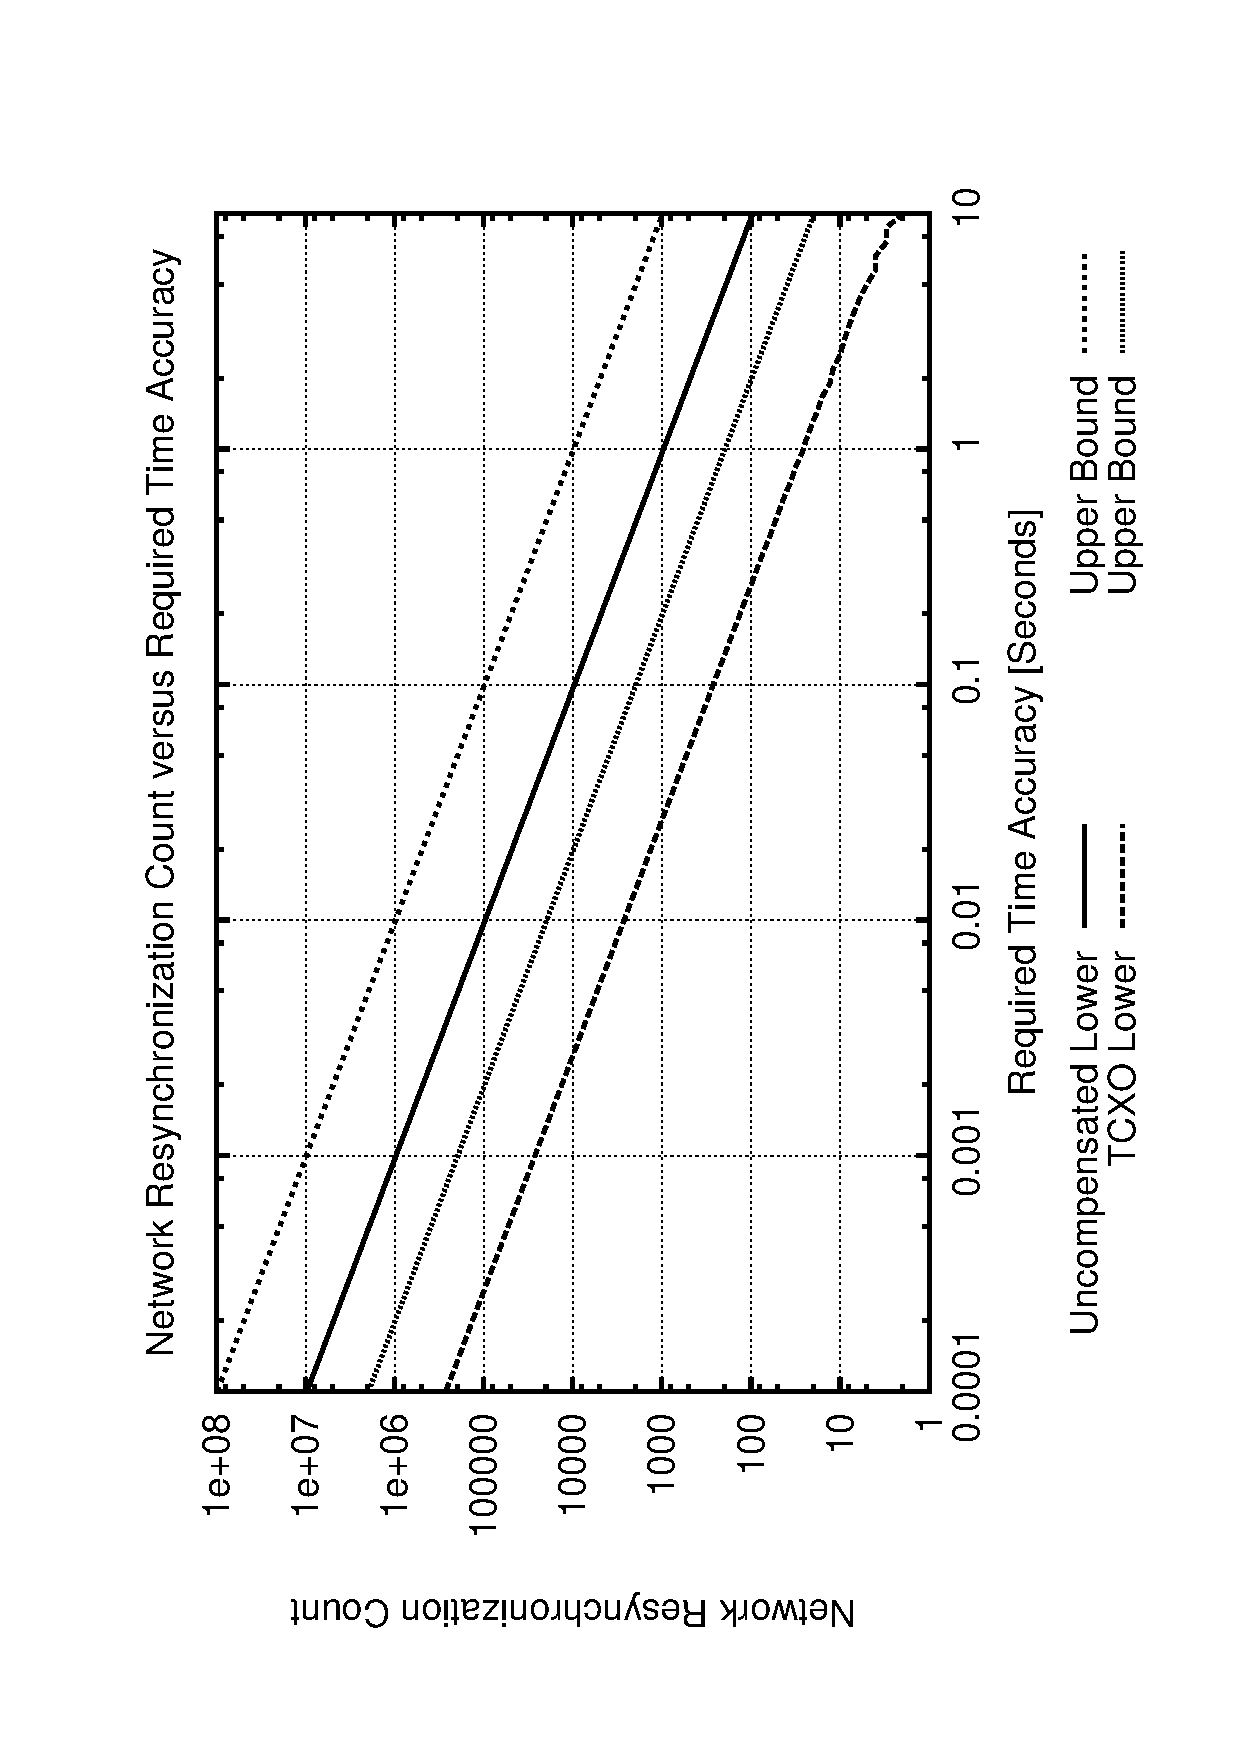
\includegraphics[angle=-90,width=0.45\textwidth]{figures/mosscamresync}
        \caption{Upper and lower bounds for the number of resynchronizations
        necessary to achieve a given time synchronization error. The
        temperature data comes from a 3 year dataset.}
        \label{fig:resync}
    \end{center}
\end{figure}

The question that arises is what would the optimal resynchronization interval be
that guarantees that synchronization error is bounded by
$\epsilon$? Assuming the system has access to an oracle that issues
the current synchronization error, and that the system does not compensate for
local clock drift, it is clear that a system with a lower drift clock will
resynchronize less often than one with a higher drift. Figure \ref{fig:resync}
illustrates this by using a 3 year temperature dataset collected at the James
Natural Wildlife Reserve \cite{mosscam}. It shows the upper and lower bounds
by calculating how often a system would have to resynchronize experiencing the
temperature changes recorded in the dataset. Looking at a specific example,
we can calculate the bandwidth savings a better clock stability can achieve.
Let's assume that the application needs a synchronization accuracy of
$\epsilon<1ms$. Over the 3 year period, an uncompensated clock would have to
resynchronize at least 900'000 times, whereas a compensated
TCXO only 25'000 times. Now, assuming that each resynchronization consists of
2 messages of 16 bytes each, results in an average bandwidth of 2.35 bit/s for
the uncompensated clock, and only 0.065 bit/s for a compensated clock.

Even though this shows that a compensated clock can lower the number of
necessary resynchronizations, it does not mean that a time synchronization
system needs to employ a TCXO to achieve this compensation. Maroti et al.
showed in \cite{maroti2004ftsp} that FTSP can estimate the current clock drift
below an accuracy of 0.1ppm. Thus, as long as the environment temperature
doesn't change too often, drift compensation can be achieved in software to a
very high accuracy.

